\chapter{Experimente}
In diesem Kapitel werden wir drei verschiedenen Beispielen mit sämtliche eingeführten Methoden duchrechnen. Dabei wird zunächst auf die Lösung der Differentialgleichung eingegangen und Konvergenzbetrachtungen durchgeführt. Danach wird der Gradienten des Kostenfunktionals behandelt und die Optimierung für diverse Anfangswerte durchgeführt. %Stay Tuned!
\section{Rolling Stone}
\subsection{Problemstellung}
Zum Anfang wollen wir uns dem sogenannten Rolling Stones Beispiel widmen, welches beispielsweise in \cite{boeck2014experiments} oder \cite{hasenfelder13} behandelt wurde. 
Es behandelt eine sich reibungslos bewegende Kugel auf einer konvexen Parabel, in dessen Mitte eine flache Ebene auf dem Intervall $[-1,1]$ eingefügt wurde. 
\begin{figure}[ht]
\centering
\begin{minipage}[b]{0.49\linewidth}
% \begin{minipage}[t][3cm][t]{5cm}
\documentclass{standalone}
\IfStandalone{
	\usepackage{pgfplots,pgfplotstable}
	\usetikzlibrary{external}
	
	}{%
}
% \usepackage{pgfplots,pgfplotstable}
% \usetikzlibrary{external}
	

\begin{document}
\tikzsetnextfilename{rolling-stones}
\begin{tikzpicture}[x=3em,y=3em]
\begin{axis}[
            xmin=-2.5,xmax=2.5,
            ymin=-1.5,ymax=1.5,
            xlabel=$z$,
%             legend entries={$V(z)$,$V'(z)$},
            width=\linewidth
        ]
        \addplot[domain=-2.5:-1]{(1+x)^2/2};
        \addplot[-,domain=-1:1]{0};
        \addplot[domain=1:2.5]{(1-x)^2/2};
        \addplot[domain=-2.5:2.5,samples=100,blue]{-min(max(-1-x,0),1-x)};
\end{axis}
\end{tikzpicture}

 
\end{document}

\caption{Rolling Stones}
\label{fig:rollingStones}
\end{minipage}
% \quad
\begin{minipage}[b]{0.49\linewidth}
% \begin{minipage}[t][3cm][t]{5cm}
\documentclass{standalone}
\IfStandalone{
	\usepackage{pgfplots,pgfplotstable}
	\usetikzlibrary{external}
	
	}{%
}
\begin{document}
\tikzsetnextfilename{rolling-stones-solution}
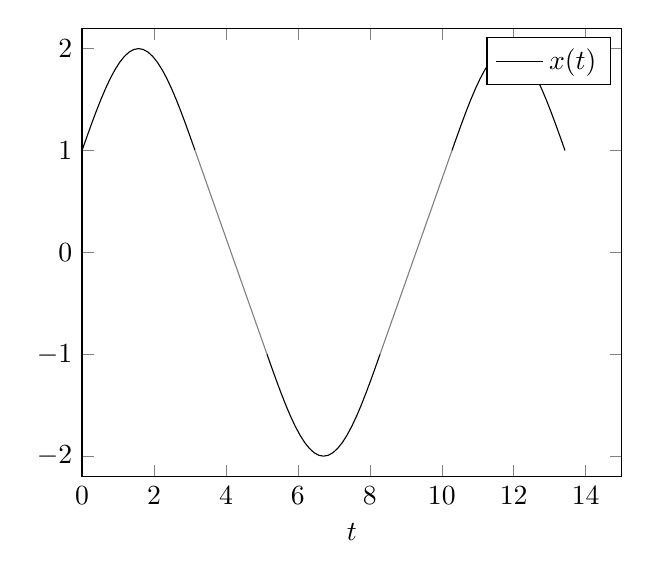
\begin{tikzpicture}[x=3em,y=3em]
\begin{axis}[
            xmin=0,xmax=15,
            ymin=-2.2,ymax=2.2,
            xlabel=$t$,
            legend entries={$x(t)$}
        ]
        \addplot[domain=0:3.14]{1+sin(deg(x))};
        \addplot[domain=pi:pi+2,gray]{1-x+pi};
        \addplot[domain=pi+2:2*pi+2]{-1-sin(deg(2-x))};
        \addplot[domain=2*pi+2:2*pi+4,gray]{x-3-2*pi};
        \addplot[domain=2*pi+4:3*pi+4]{1+sin(deg(x-2*pi-4))};
\end{axis}
\end{tikzpicture} 
\end{document}

\caption{Rolling Stones Lösung}
\label{fig:rollingStonesSolution}
\end{minipage}
\end{figure}
Figur \ref{fig:rollingStones} zeigt die Rampe
\[
 V(z) = \left(\frac{(1+z)^2}{2}\right)\chi_{(-\infty,-1]} + \left(\frac{(1-z)^2}{2}\right)\chi_{[1,\infty)} ,
 ~ \chi_{[a,b)}(z) = 
 \begin{cases}
  1 & z \in [a,b)\\
  0 & \text{sonst}
 \end{cases}
\]

und deren Ableitung, welche wir als gewöhnliche Differentialgleichung
 \begin{equation}
  \begin{pmatrix}
   \dot x_1 \\
   \dot x_2 \\
  \end{pmatrix}
 = 
 \begin{pmatrix}
  x_2 \\
  -x_1 - \frac{|x_1-1|}{2} + \frac{|x_1+1|}{2}
 \end{pmatrix}
=F(x)
\label{eq:rolling_stones}
 \end{equation}
auffassen, wobei $x_1$ die Abszissenposition des Steines und $x_2$ dessen Geschwindigkeit bezeichnet.
Die Funktion \eqref{eq:rolling_stones} ist stückweise linear, sodass wir seine Abs Normal Form \eqref{eq:absNormalForm} angeben können mit
\[
c = \begin{pmatrix}
     -1\\
     1
    \end{pmatrix}
\quad
 Z = \begin{pmatrix}
      1 & 0 \\
      1 & 0
     \end{pmatrix}\quad
J = \begin{pmatrix}
      0&1\\
      -1 & 0
     \end{pmatrix}\quad
 Y = \begin{pmatrix}
      0 & 0\\
      -0.5  & 0.5
     \end{pmatrix}
\]
der Rest wird passend zur Dimension zu $0$ gesetzt. Für das Rolling Stones Beispiel lässt sich eine analytische Lösung zur ODE \eqref{eq:rolling_stones} für den Anfangswert $x_0=(1,1)$ angeben. Sie ist $2\pi+4$ periodisch, hat die Form
\begin{equation}
 x(t) = \begin{cases}
         1+\sin(t) 	& 0\leq t \leq \pi	\\
         1-(t-\pi) 	& \pi \leq t < \pi+2	\\ 
         -1 - \sin(2-t) 	& \pi+2\leq t<2\pi+2	\\
         t-3-2\pi	& 2\pi+2 \leq t<2\pi +4
        \end{cases}
\label{eq:analyticSolRolling}
\end{equation}
und wird in Figur \ref{fig:rollingStonesSolution} angegeben. Dabei sind die grau eingezeichneten Bereiche linear.

\subsection{Lösen der ODE}
Die Konvergenz der verallgemeinerten impliziten Mittelpunktsregel 
\begin{figure}
\centering
\documentclass{standalone}
\IfStandalone{
	\usepackage{pgfplots,pgfplotstable}
	\usetikzlibrary{external}
	\newcommand{\fromRoot}[1]{../#1}
}{%
}
\begin{document}
\tikzsetnextfilename{convergence_rolling_plot}
\begin{tikzpicture}
\begin{loglogaxis}[
	width=10cm,
	xlabel=Degrees of freedom $N$,
	ylabel=Error at time $T$,
	legend entries ={Expl. MP,
	IMP,
	GIMP, 
	}
]
  	\addplot[mark=none,red,very thin] table[x index=0,y index=2] {img/data/convergence_rolling_plot.dat};%expl midpoint
 	\addplot[mark=none,green,very thin] table[x index=0,y index=3] {img/data/convergence_rolling_plot.dat};%impl midpoint
	\addplot[mark=none,blue,very thin] table[x index=0,y index=1] {img/data/convergence_rolling_plot.dat};%gen midpoint

	\addplot[mark=none,very thin,gray, yshift=-20pt] 
		table[y={create col/linear regression={x=0,y=1}}] {img/data/convergence_rolling_plot.dat}
		  coordinate [pos=0.5] (A)
		  coordinate [pos=0.6] (B)
		;
	% save the slope parameter:
	\pgfmathparse{-\pgfplotstableregressiona}	
	\pgfmathsetmacro{\slope}{\pgfmathresult}
	
	% draw the opposite and adjacent sides
	% of the triangle
	\draw[very thin,gray] (B) -| (A)
	node [pos=0.2,anchor=north]
	{\pgfmathprintnumber{\slope}};
\end{loglogaxis}
\end{tikzpicture}
\end{document}
\caption{Konvergenz Rolling Stones im Intervall $[0,50]$ mit $x_0=(1,1)$}
\label{fig:rollingStonesConvergence}
\end{figure}


\begin{figure}[H]
\footnotesize 
\centering
% \quad
\begin{minipage}[b]{0.45\linewidth}
% \begin{minipage}[t][3cm][t]{5cm}
\documentclass{standalone}
\IfStandalone{
	\usepackage{pgfplots,pgfplotstable}
	\usetikzlibrary{external}
	\newcommand{\fromRoot}[1]{../#1}
}{%
}

\begin{document}
\tikzsetnextfilename{rolling_energy_error}
\begin{tikzpicture}
\begin{loglogaxis}[
	width=\linewidth,
	xlabel=Anzahl der Freiheitsgrade $N$,
	ylabel=Mittelwert des Energieverlustes,
	legend entries ={Expl. MP,
	IMP,
	GIMP 
	},
	legend style={at={(0.5,1.0)},anchor=south},
	legend columns=2
]
  	\addplot[mark=none,red,very thin] table[x index=0,y index=2] {\fromRoot img/data/rolling_energy_error.dat};%expl midpoint
 	\addplot[mark=none,green,very thin] table[x index=0,y index=3] {\fromRoot img/data/rolling_energy_error.dat};%impl midpoint
	\addplot[mark=none,blue,very thin] table[x index=0,y index=1] {\fromRoot img/data/rolling_energy_error.dat};%gen midpoint
\end{loglogaxis}
\end{tikzpicture}
\end{document}
\caption{Rolling Stones Energieverlust im Intervall $[0,2\pi+4]$ mit $x_0=(1,1)$}
\label{fig:rollingStonesEnergyError}
\end{minipage}
\quad
\begin{minipage}[b]{0.45\linewidth}
% \begin{minipage}[t][3cm][t]{5cm}
\documentclass{standalone}
\IfStandalone{
	\usepackage{pgfplots,pgfplotstable}
	\usetikzlibrary{external}
	\newcommand{\fromRoot}[1]{../#1}
}{%
}
\begin{document}
\tikzsetnextfilename{convergence_rolling_romberg_plot}
\begin{tikzpicture}
\begin{loglogaxis}[
	width=10cm,
	xlabel=Anzahl der Freiheitsgrade $N$,
	ylabel=Fehler in $x$,
% 	title=Convergence of SWE,
	legend entries ={
% 	Expl. MP,
	IMP,
	GIMP, 
	Romberg Impl,
	Romberg Gen
	}
]
 	\addplot[mark=none,green,very thin] table[x index=0,y index=3] {img/data/convergence_rolling_romberg_plot.dat};%impl midpoint
	\addplot[mark=none,blue,very thin] table[x index=0,y index=1] {img/data/convergence_rolling_romberg_plot.dat};%gen midpoint

	\addplot[mark=none,lime,very thin] table[x index=0,y index=5] {img/data/convergence_rolling_romberg_plot.dat};%Romberg impl midpoint
	\addplot[mark=none,cyan,very thin] table[x index=0,y index=4] {img/data/convergence_rolling_romberg_plot.dat};%ROMBERG gen midpoint
	
	
	\addplot[mark=none,very thin,gray, yshift=-20pt] 
		table[y={create col/linear regression={x=0,y=4}}] {img/data/convergence_rolling_romberg_plot.dat}
		  coordinate [pos=0.5] (A)
		  coordinate [pos=0.6] (B)
		;
	% save the slope parameter:
	\pgfmathparse{-\pgfplotstableregressiona}	
	\pgfmathsetmacro{\slope}{\pgfmathresult}
	
	% draw the opposite and adjacent sides
	% of the triangle
	\draw[very thin,gray] (B) -| (A)
	node [pos=0.2,anchor=north]
	{\pgfmathprintnumber{\slope}};
\end{loglogaxis}
\end{tikzpicture}
\end{document}
\caption{Konvergenz der Romberg Extrapolation im Intervall $[0,50]$ mit $x_0=(1,1)$}
\label{fig:rollingStonesConvergenceRomberg}
\end{minipage}

\end{figure}


Die in Theorem \ref{thm:convergenceGenMidpoint} vorhergesagte Konvergenzordnung von $\mathcal O(h^2)$ erfüllt die verallgemeinerte implizite Mittelpunktsregel wie in Figur \ref{fig:rollingStonesConvergence} ersichtlich.
Dass die gewöhnliche implizite Mittelpunktsregel eine ebenso hohe Konvergenzrate besitzt ist darin begründet, dass sie im gegebenen Intervall nur $4$ mal pro $2\pi+4$ Periode Unglattheiten überquert, sonst jedoch normal konvergiert. Aufgrund dieser Unglattheiten entsteht für die implizite Mittelpunktsregel (IMP) kein glatter Konvergenzgraph, sondern sie springt. Demgegenüber konvergiert die verallgemeinerter implizite Mittelpunktsregel (GIMP) sehr stabil, da sie die Knicke der Funktion mit in ihre Berechnung einbezieht.
Insbesondere wird der Fehler der GIMP mit zunehmender Zeit (siehe Fig. \ref{fig:rollingStonesEOT}) nur in den nicht affinen Abschnitten größer während in den affinen Abschnitten exakt gelöst wird, der lokale Fehler der IMP erhöht sich jedoch ständig, bedingt durch die Kinks und der zu großen Schrittweite. Der allgemeine Fehler ist dadurch für die IMP höher über die Zeit gesehen als der Fehler der GIMP (\ref{fig:rollingStonesEOTAll}).

Da sich der rollende Stein reibungslos in unserem System bewegt, muss die analytische Lösung die komplette Energie erhalten, d.h. die potentielle Energie addiert mit der kinetischen $V(x) + \frac{1}{2}\dot x^2$ muss konstant sein. Das Bild \ref{fig:rollingStonesEnergyError} wurde mittels der summierten Variation der Energie 
\[
 h \left[\sum_{l=0}^{T/h} \left( V(x_1^l) + \frac{1}{2} (x_2^l)^2 -\frac{1}{2}\right)^2\right]^{\sfrac{1}{2}}
\]
berechnet. Es ist deutlich zu erkennen, dass die Energie mit der GIMP deutlich besser erhalten bleibt als mit den klassischen Methoden, selbst für große Schrittweiten.
Dadurch führt die in Figur \ref{fig:rollingStonesConvergenceRomberg} durchgeführte Romberg Extrapolation zu sehr guten Ergebnissen. Da der Konvergenzgraph der GIMP stabil ist, lässt sich eine gute Extrapolation mit Konvergenzen der Ordnung 3 bis 4 erreichen. Demgegebenüber besitzt die Extrapolation der IMP keine höhere Konvergenzordnung als die der IMP selbst.
\begin{figure}[H]
\footnotesize 
\centering
\begin{minipage}[b]{0.49\linewidth}
% \begin{minipage}[t][3cm][t]{5cm}
\documentclass{standalone}
\IfStandalone{
	\usepackage{pgfplots,pgfplotstable}
	\usetikzlibrary{external}
	\newcommand{\fromRoot}[1]{../#1}
}{%
}
\begin{document}
\tikzsetnextfilename{rolling_error_over_time}
\begin{tikzpicture}
\begin{axis}[
	width=\linewidth,
	xlabel=Zeitpunkt $t$,
	ylabel=Fehler zum Zeitpunkt $t$,
	legend entries ={Expl. MP,
	IMP,
	GIMP, 
	},
	legend style={at={(0,1)},anchor=north west}
]
\addplot[mark=none,red,very thin] table[x index=0,y index=3] {img/data/rolling_error_over_time.dat};
\addplot[mark=none,green,very thin] table[x index=0,y index=2] {img/data/rolling_error_over_time.dat};
\addplot[mark=none,blue,very thin] table[x index=0,y index=1] {img/data/rolling_error_over_time.dat};

\end{axis}
\end{tikzpicture}
\end{document}
\caption{Rolling Stones Fehler über Zeit, \\$h=0.1,x_0=(1,1)$}
\label{fig:rollingStonesEOT}
\end{minipage}
% \quad
\begin{minipage}[b]{0.49\linewidth}
% \begin{minipage}[t][3cm][t]{5cm}
\documentclass{standalone}
\IfStandalone{
	\usepackage{pgfplots,pgfplotstable}
	\usetikzlibrary{external}
	\newcommand{\fromRoot}[1]{../#1}
}{%
}
\begin{document}
\tikzsetnextfilename{rolling_error_over_time_all}
\begin{tikzpicture}
\begin{axis}[
	width=\linewidth,
	xlabel=Zeitpunkt $t$,
	ylabel=Fehler über alle Komponenten,
	legend entries ={Expl. MP,
	IMP,
	GIMP 
	},
% 	legend style={at={(0,1)},anchor=north west}
	legend style={at={(0.5,1.0)},anchor=south},
	legend columns=2
]
\addplot[mark=none,red,very thin] table[x index=0,y index=3] {img/data/rolling_error_over_time_all.dat};
\addplot[mark=none,green,very thin] table[x index=0,y index=2] {img/data/rolling_error_over_time_all.dat};
\addplot[mark=none,blue,very thin] table[x index=0,y index=1] {img/data/rolling_error_over_time_all.dat};

\end{axis}
\end{tikzpicture}
\end{document}
\caption{Rolling Stones Fehler über alle Komponenten, $h=0.1,x_0=(1,1)$}
\label{fig:rollingStonesEOTAll}
\end{minipage}
\end{figure}

\subsection{Gradient des Kostenfunktionals}
Ähnliche Ergebnisse wie beim Lösen der ODE erwarten wir für die Integration des inhomogenen adjungierten Tangent Linear Models \eqref{eq:inhAdjEquation}. Falls nicht anders beschrieben werden im Folgenden immer die exakte Lösung des Rolling Stones Beispiel \eqref{eq:analyticSolRolling} als Obervierungsparameter $x_{\text{Obs}}$ mit der selben Diskretisierung wie die des ODE Lösers verwendet.

Beim Plot des Gradienten nach Anfangswerten wie in Figur \ref{fig:rollingGrad} ist zu erkennen, dass der Gradient berechnet mit der GIMP ebenfalls stabiler wirkt (Fig. \ref{fig:rollingGrad} links) als der Gradient berechnet mit der normalen Impliziten Mittelpunktsregel (Fig. \ref{fig:rollingGrad} rechts). Desweiteren existieren im Letzteren vereinzelt hohe Sprünge, welche durch nicht einbezogene Kinks erklärt werden können. 
\begin{figure}[H]
\footnotesize 
\centering
\begin{minipage}[b]{0.49\linewidth}
% \begin{minipage}[t][3cm][t]{5cm}
\documentclass{standalone}
\usepackage{pgfplots,pgfplotstable}
\IfStandalone{
	\usepackage{pgfplots,pgfplotstable}
	\usetikzlibrary{external}
	\newcommand{\fromRoot}[1]{../#1}
}{%
}
\begin{document}
\tikzsetnextfilename{rolling_jac_da_gradient1}
\begin{tikzpicture}
    \begin{axis}[view={-20}{60}, grid=both,width=\linewidth,
%      title={$\sfrac{\partial J}{\partial x_0^{(1)}}$},
    xlabel={$x_0^{(0)}$},
    ylabel={$x_0^{(1)}$},
    zlabel={$\sfrac{\partial J}{\partial x_0^{(1)}}$}]
      \addplot3[surf] file {img/data/grad1_gimp.dat};
    \end{axis}
\end{tikzpicture}
\end{document}
% \caption{Rolling Stones Fehler über Zeit}
% \label{fig:rollingGrad1Gimp}
\end{minipage}
% \quad
\begin{minipage}[b]{0.49\linewidth}
% \begin{minipage}[t][3cm][t]{5cm}
\documentclass{standalone}
\IfStandalone{
	\usepackage{pgfplots,pgfplotstable}
	\usetikzlibrary{external}
	\newcommand{\fromRoot}[1]{../#1}
}{%
}
\begin{document}
\tikzsetnextfilename{rolling_jac_da_gradient1_imp}
\begin{tikzpicture}
    \begin{axis}[view={-20}{60}, grid=both,width=\linewidth,
%      title={$\sfrac{\partial J}{\partial x_0^{(1)}}$},
    xlabel={$x_0^{(0)}$},
    ylabel={$x_0^{(1)}$},
    zlabel={$\sfrac{\partial J}{\partial x_0^{(1)}}$}]
      \addplot3[surf] file {\fromRoot img/data/grad1_impl.dat};
    \end{axis}
\end{tikzpicture}
\end{document}
% \caption{Rolling Stones Fehler über alle Komponenten}
% \label{fig:rollingGrad1Imp}
\end{minipage}
\begin{minipage}[b]{0.49\linewidth}
% \begin{minipage}[t][3cm][t]{5cm}
\documentclass{standalone}
\IfStandalone{
	\usepackage{pgfplots,pgfplotstable}
	\usetikzlibrary{external}
	\newcommand{\fromRoot}[1]{../#1}
}{%
}
\begin{document}
\tikzsetnextfilename{rolling_jac_da_gradient2}
  \begin{tikzpicture}
    \begin{axis}[view={-20}{60}, grid=both,width=\linewidth,
%      title={$\sfrac{\partial J}{\partial x_0^{(1)}}$},
    xlabel={$x_0^{(0)}$},
    ylabel={$x_0^{(1)}$},
    zlabel={$\sfrac{\partial J}{\partial x_0^{(1)}}$}]
      \addplot3[surf] file {img/data/grad2_gimp.dat};
      
    \end{axis}
\end{tikzpicture}
\end{document}
% \caption{Ableitung des Kostenfunktional in erster Komponente von Rolling Stones }
% \label{fig:rollingGrad2Gimp}
\end{minipage}
% \quad
\begin{minipage}[b]{0.49\linewidth}
% \begin{minipage}[t][3cm][t]{5cm}
\documentclass{standalone}
\IfStandalone{
	\usepackage{pgfplots,pgfplotstable}
	\usetikzlibrary{external}
	\newcommand{\fromRoot}[1]{../#1}
}{%
}
\begin{document}
\tikzsetnextfilename{rolling_jac_da_gradient2_imp}
  \begin{tikzpicture}
    \begin{axis}[view={-20}{60}, grid=both,width=\linewidth,
%      title={$\sfrac{\partial J}{\partial x_0^{(1)}}$},
    xlabel={$x_0^{(0)}$},
    ylabel={$x_0^{(1)}$},
    zlabel={$\sfrac{\partial J}{\partial x_0^{(1)}}$}]
      \addplot3[surf] file {img/data/grad2_impl.dat};
      
    \end{axis}
\end{tikzpicture}
\end{document}
% \caption{Ableitung des Kostenfunktional in erster Komponente von Rolling Stones}
% \label{fig:rollingGrad2Imp}
\end{minipage}
\caption{Ableitung des Kostenfunktionals beim Rolling Stones Beispiel (links: GIMP, rechts: IMP), $I = [0,30],h=0.5$}
\label{fig:rollingGrad}
\end{figure}


Die Konvergenzplots \ref{fig:rollingStonesAdjointSmooth} und \ref{fig:rollingStonesAdjointDiscrete} ergeben ähnliche Robustheitsresultate wie bei der Vorwärtsintegration. Figur \ref{fig:rollingStonesAdjointSmooth} stellt dabei die Konvergenz mit einer Funktion als Observierungsparameter dar. Das bedeutet, dass in jeder Verfeinerung ebenfalls die Observierungsparameter verfeinert wurden also $t_{\text{state}} = t_{\text{Obs}}$. Diskrete Observierungsparameter wurden bei Figur \ref{fig:rollingStonesAdjointDiscrete} benutzt, sie blieben also bei jeder Verfeinerung des Gitters konstant. Die aus der GIMP berechneten Werte wurden mit einem Projektionsoperator vom Zustandsraum $X_{\text{State}}$ in den Raum der Observierungen $X_{\text{Obs}}$ projeziert, danach deren Differenz gebildet und wieder zurück nach $X_{\text{State}}$ projeziert. Die lineare Konvergenz der beiden Plots liefert 



Dabei fällt die lineare Konvergenz aller Methoden auf. Selbst für einfachere Beispiele ohne Kinks ist die Konvergenz nicht schneller als linear.
TODO: HERAUSFINDEN WARUM DAS SO IST


\begin{figure}[H]
\footnotesize 
\centering
\begin{minipage}[b]{0.49\linewidth}
% \begin{minipage}[t][3cm][t]{5cm}
\documentclass{standalone}
\IfStandalone{
	\usepackage{pgfplots,pgfplotstable}
	\usetikzlibrary{external}
	\newcommand{\fromRoot}[1]{../#1}
}{%
}
\begin{document}
\tikzsetnextfilename{rolling_convergence_adjoint_smooth}
\begin{tikzpicture}
\begin{loglogaxis}[
	width=\linewidth,
	xlabel=Anzahl der Freiheitsgrade $N$,
	ylabel=Fehler in $x$,
	legend entries ={Expl. MP,
	IMP,
	GIMP, 
	}
]
  	\addplot[mark=none,red,very thin] table[x index=0,y index=3] {img/data/rolling_convergence_adjoint_smooth.dat};%expl midpoint
 	\addplot[mark=none,green,very thin] table[x index=0,y index=2] {img/data/rolling_convergence_adjoint_smooth.dat};%impl midpoint
	\addplot[mark=none,blue,very thin] table[x index=0,y index=1] {img/data/rolling_convergence_adjoint_smooth.dat};%gen midpoint

	\addplot[mark=none,very thin,gray, yshift=-20pt] 
		table[y={create col/linear regression={x=0,y=1}}] {img/data/rolling_convergence_adjoint_smooth.dat}
		  coordinate [pos=0.2] (A)
		  coordinate [pos=0.3] (B)
		;
	% save the slope parameter:
	\pgfmathparse{-\pgfplotstableregressiona}	
	\pgfmathsetmacro{\slope}{\pgfmathresult}
	
	% draw the opposite and adjacent sides
	% of the triangle
	\draw[very thin,gray] (B) -| (A)
	node [pos=0.17,anchor=north]
	{\pgfmathprintnumber{\slope}};
\end{loglogaxis}
\end{tikzpicture}
\end{document}
\caption{Rolling Stones Konvergenz glatt\\ $I=[0,40]$}
\label{fig:rollingStonesAdjointSmooth}
\end{minipage}
% \quad
\begin{minipage}[b]{0.49\linewidth}
% \begin{minipage}[t][3cm][t]{5cm}
\documentclass{standalone}
\IfStandalone{
	\usepackage{pgfplots,pgfplotstable}
	\usetikzlibrary{external}
	\newcommand{\fromRoot}[1]{../#1}
}{%
}
\begin{document}
\tikzsetnextfilename{rolling_convergence_adjoint_discrete}
\begin{tikzpicture}
\begin{loglogaxis}[
	width=\linewidth,
	xlabel=Anzahl der Freiheitsgrade $N$,
	ylabel=Fehler in $x$,
	legend entries ={Expl. MP,
	IMP,
	GIMP, 
	}
]
  	\addplot[mark=none,red,very thin] table[x index=0,y index=3] {img/data/rolling_convergence_adjoint_discrete.dat};%expl midpoint
 	\addplot[mark=none,green,very thin] table[x index=0,y index=2] {img/data/rolling_convergence_adjoint_discrete.dat};%impl midpoint
	\addplot[mark=none,blue,very thin] table[x index=0,y index=1] {img/data/rolling_convergence_adjoint_discrete.dat};%gen midpoint

	\addplot[mark=none,very thin,gray, yshift=-20pt] 
		table[y={create col/linear regression={x=0,y=1}}] {img/data/rolling_convergence_adjoint_discrete.dat}
		  coordinate [pos=0.2] (A)
		  coordinate [pos=0.3] (B)
		;
	% save the slope parameter:
	\pgfmathparse{-\pgfplotstableregressiona}	
	\pgfmathsetmacro{\slope}{\pgfmathresult}
	
	% draw the opposite and adjacent sides
	% of the triangle
	\draw[very thin,gray] (B) -| (A)
	node [pos=0.2,anchor=north]
	{\pgfmathprintnumber{\slope}};
\end{loglogaxis}
\end{tikzpicture}
\end{document}
\caption{Rolling Stones Konvergenz diskret\\ $I=[0,40]$}
\label{fig:rollingStonesAdjointDiscrete}
\end{minipage}
\end{figure}

\subsection{Optimierung}
Die zu minimierende Funktion, das Kostenfunktional $J$, ist in Figur \ref{fig:rolling_costfunctional} gegeben. $J$ ist hierbei offensichtlich nicht konvex; es entsteht um den Punkt $(0,0)$ eine Art Spirale. Sein Minimum befindet sich am Punkt $(1,1)$, trivialerweise an der Stelle der Observierungsparameter. 
% Pfad der Iterationen
\begin{figure}[H]
\centering
\documentclass{standalone}
\usepackage{pgfplots,pgfplotstable}
\IfStandalone{
	\usepackage{pgfplots,pgfplotstable}
	\usetikzlibrary{external}
	\newcommand{\fromRoot}[1]{../#1}
}{%
}
\begin{document}
\tikzsetnextfilename{rolling_costfunctional}
\begin{tikzpicture}
    \begin{axis}[view={-20}{60}, grid=both,width=12cm,
%      title={$\sfrac{\partial J}{\partial x_0^{(1)}}$},
    xlabel={$x_0^{(0)}$},
    ylabel={$x_0^{(1)}$},
    zlabel={$J(x_0)$}]
      \addplot3[surf] file {img/data/rolling_costfunctional.dat};
    \end{axis}
\end{tikzpicture}
\end{document}
\caption{Rolling Stones Kostenfunktional im Intervall $[0,30],h=0.5$}
\label{fig:rolling_costfunctional}
\end{figure}

Die Optimierung in diesem Beispiel wurden mit dem BFGS - Verfahren (siehe Algorithmus \ref{alg:bfgs}) durchgeführt. Dabei war in den Versuchen zu erkennen, dass die verallgemeinerte Methode ein besseres Konvergenzverhalten durch den glatteren Gradienten besitzt (Figur \ref{fig:rollingStonesOpt2}).

Für bestimmte Anfangswerte divergiert die klassische Methode wie in Figur \ref{fig:rollingStonesOpt1} wohingegen die Optimierung über GIMP konvergiert. 

Zusammenfassend ergibt sich für das Rolling Stones Beispiel ein insgesamt besseres Verhalten der verallgemeinerten Methoden im Gegensatz zu der klassischen impliziten Mittelpunktsregel.
\begin{figure}[H]
\footnotesize
\centering
\begin{minipage}[b]{0.49\linewidth}
% \begin{minipage}[t][3cm][t]{5cm}
\documentclass{standalone}
\usepackage{pgfplots,pgfplotstable}
\IfStandalone{
	\usepackage{pgfplots,pgfplotstable}
	\usetikzlibrary{external}
	\newcommand{\fromRoot}[1]{../#1}
}{%
}
\begin{document}
\tikzsetnextfilename{rolling_opt2_cost}
\begin{tikzpicture}
    \begin{axis}[view={0}{90},
    width=\linewidth,
    legend entries ={Kostenfunktional,IMP, GIMP},
    legend style={at={(0.97,1.40)}},
%     legend style={at={(1.00,0.15)},anchor=east}
    xlabel={$x_0^{(0)}$},
    ylabel={$x_0^{(1)}$},
    zlabel={$\sfrac{\partial J}{\partial x_0^{(1)}}$}]
%     \addplot3[surf] file {img/data/rolling_costfunctional.dat};
     \addplot3[contour gnuplot] file {img/data/rolling_costfunctional.dat};
    \addplot3[mark=o, red] table {img/data/rolling_opt2_iterationSteps.dat};
    \addplot3[mark=o, yellow] table {img/data/rolling_opt2_iterationSteps_impl.dat};
        \end{axis}
\end{tikzpicture}
\end{document}
\end{minipage}
% \quad
\begin{minipage}[b]{0.49\linewidth}
% \begin{minipage}[t][3cm][t]{5cm}
\documentclass{standalone}
\usepackage{pgfplots,pgfplotstable}
\IfStandalone{
	\usepackage{pgfplots,pgfplotstable}
	\usetikzlibrary{external}
	\newcommand{\fromRoot}[1]{../#1}
}{%
}
\begin{document}
\tikzsetnextfilename{rolling_opt2_convergence}
\begin{tikzpicture}
\begin{loglogaxis}[
	width=\linewidth,
	xlabel=Optimierungsschritte,
	ylabel=Fehler,
% 	title=Convergence of Optimization for Rolling Stones,
	legend entries ={IMP,GIMP},
	legend style={at={(0.5,1.0)},anchor=south},
	legend columns=2
]
 	\addplot[mark=none,green,very thin] table[x index=0,y index=2] {img/data/rolling_opt2_convergence.dat};%impl midpoint
	\addplot[mark=none,blue,very thin] table[x index=0,y index=1] {img/data/rolling_opt2_convergence.dat};%gen midpoint
 \end{loglogaxis}
\end{tikzpicture}

\end{document}
\end{minipage}
\caption{Rolling Stones Data Assimilation Optimierung mit $x_0=(0,-1.45)$ auf dem Intervall $I = [0,20], h=0.2$}
\label{fig:rollingStonesOpt2}
\end{figure}

\begin{figure}[H]
\footnotesize 
\centering
\begin{minipage}[b]{0.49\linewidth}
% \begin{minipage}[t][3cm][t]{5cm}
\documentclass{standalone}
\usepackage{pgfplots,pgfplotstable}
\IfStandalone{
	\usepackage{pgfplots,pgfplotstable}
	\usetikzlibrary{external}
	\newcommand{\fromRoot}[1]{../#1}
}{%
}
\begin{document}
\tikzsetnextfilename{rolling_opt1_cost}
\begin{tikzpicture}
    \begin{axis}[view={0}{90},
    width=\linewidth,
    legend entries ={Kostenfunktional,IMP, GIMP},
    legend style={at={(0.97,1.40)}},
%     legend style={at={(1.00,0.15)},anchor=east}
    xlabel={$x_0^{(0)}$},
    ylabel={$x_0^{(1)}$},
    zlabel={$\sfrac{\partial J}{\partial x_0^{(1)}}$}]
%     \addplot3[surf] file {img/data/rolling_costfunctional.dat};
     \addplot3[contour gnuplot={number=5}] file {img/data/rolling_costfunctional.dat};
    \addplot3[mark=o, green] table {img/data/rolling_opt1_iterationSteps_impl.dat};
    \addplot3[mark=o, blue] table {img/data/rolling_opt1_iterationSteps.dat};
    \end{axis}
\end{tikzpicture}
\end{document}
\end{minipage}
% \quad
\begin{minipage}[b]{0.49\linewidth}
% \begin{minipage}[t][3cm][t]{5cm}
\documentclass{standalone}
\usepackage{pgfplots,pgfplotstable}
\IfStandalone{
	\usepackage{pgfplots,pgfplotstable}
	\usetikzlibrary{external}
	\newcommand{\fromRoot}[1]{../#1}
}{%
}
\begin{document}
\tikzsetnextfilename{rolling_opt1_convergence}
\begin{tikzpicture}
\begin{loglogaxis}[
	width=\linewidth,
	xlabel=Optimierungsschritte,
	ylabel=Fehler,
% 	title=Convergence of Optimization for Rolling Stones,
	legend entries ={IMP,GIMP},
	legend style={at={(0.87,1.28)}}
]
  	
 	\addplot[mark=none,green,very thin] table[x index=0,y index=2] {img/data/rolling_opt1_convergence.dat};%impl midpoint
\addplot[mark=none,blue,very thin] table[x index=0,y index=1] {img/data/rolling_opt1_convergence.dat};%gen midpoint
 	\end{loglogaxis}
\end{tikzpicture}

\end{document}
\end{minipage}
\caption{Rolling Stones Data Assimilation Optimierung mit $x_0=(1.5,1.5)$ auf dem Intervall $I = [0,20], h=0.2$}
\label{fig:rollingStonesOpt1}
\end{figure}


\section{LC-Diode}
\begin{figure}[H]
\centering
\documentclass{standalone}
\usepackage{pgfplots,pgfplotstable,circuitikz}

\usetikzlibrary{external}

\begin{document}

\tikzsetnextfilename{lc-circuit}
\begin{tikzpicture}[x=1.5cm]
% \draw[help lines] (0,0) grid (5,3);
% \draw (0,0) 
%     to[L] (0,3) 
%     to (2,3) 
%     to[C=$C$] (3,3)
%     to (5,3)
%     to[diode] (5,0) 
%     to (0,0);
%     to[V,v=$U_q$] (0,2) % The voltage source
\draw (0,0) 
    to (3,0)
    to[V,v=$V(t)$] (3,1.5) % The voltage source
    to[diode] (3,3) 
    to (3,3)
    to[C=$C$] (0,3)
%     to (0,3)
    to[L=$L$](0,0) 
    to (0,0);
    % \draw (2,0) to[C] (2,3);
% \draw (3,0) to[C] (3,3);
% \draw (2.5,0) node[ground] {};
\draw (2.7,2.7) node[anchor=north east,align=right] {$g(x)$};
\draw (2.1,0) node[anchor=north east,align=right] {$I(t)=z(t)$};
% \draw (1.8,1.5) node[anchor=north east] {$C_1$};
% \draw (2.8,1.5) node[anchor=north east] {$C_2$};
% \draw (-0.2,1.5) node[anchor=north east] {$L$};
\end{tikzpicture}

 
\end{document}

\caption{LC Schaltkreis Diagramm}
\label{fig:lcDiode}
\end{figure}



\cite{boeck2014experiments}
\section{Shallow Water Equation}
\subsection{Problemstellung}
\subsection{Unglattheiten}
Fluxlimiter, Eigenwerte, Plot der Rechten Seite
\subsection{Ergebnisse}


Ein oft genutztes Beispiel, um Datenassimilierungsmethoden zu testen ist die sogenannte Shallow Water Equation (vgl. \cite{zou,navon}). Diese beschreibt die Bewegung einer Flüssigkeit in einem quadratischen Gebiet unter Berücksichtigung von Gravitationswellen. In kartesischen Koordinaten erhält man folgende Gleichungen
\begin{equation}
\begin{aligned}
 \frac{\partial u }{\partial t} = -u\frac{\partial u}{\partial x} -v\frac{\partial u}{\partial y} + fv - \frac{\partial \phi}{\partial x}\\
 \frac{\partial v }{\partial t} = -u\frac{\partial v}{\partial x} -v\frac{\partial v}{\partial y} - fu - \frac{\partial \phi}{\partial y}\\
 \frac{\partial \phi }{\partial t} = -\frac{\partial u\phi}{\partial x} -\frac{\partial v\phi}{\partial y} 
\end{aligned}
\label{eq:swe}
 \end{equation}
Hierbei sind $u$ und $v$ die zwei Komponenten des Fließgeschwindigkeitsfeldes in $s^{-1}$ und $\phi$ das Geopotential in $m^2 s^{-1}$; 
$f$ bezeichnet den Coriolisfaktor.
Die Anfangsbedingungen für die folgenden Experimente wurden aus \cite{grammeltvedt}(6.I) übernommen. Es handelt sich hierbei um eine westwärtgsgerichtete Strömung mit Nord - Süd Störungen verschiedener Wellenlängen und Amplituden entlang der Zonal - Achse der Strömung. Das anfängliche Höhenfeld wurde gewählt mittels Höhenfunktion
\begin{align*}
 h(x,y) = H_0 + H_1 \tanh \left( \frac{9(y-y_0)}{2D}\right) + H_2 \sech^2\left(\frac{9(y-y_0)}{D}\right) \sin\left(\frac{2\pi x}{L}\right)
\end{align*}
und Ableitungen
\begin{align*}
 \frac{\partial h}{\partial x}(x,y) &= h_2\sech^2\left( \frac{9(y-y_0)}{D}\right) \cos\left( \frac{2\pi x}{L} \right)\frac{2\pi}{L} \\
 \frac{\partial h}{\partial y}(x,y) &= h_1 \sech^2\left( \frac{9(y-y_0)}{2D}\right)\frac{9}{2D} -  h_2\frac{18}{D} \sin\left( \frac{2\pi x}{L}\right) \frac{\sinh(9(y-y_0)/D)}{\cosh^3(9(y-y_0)/D)}\\
\end{align*}
wobei $D$ die Breite, $L$ die Länge der betrachteten Fläche ist,  $h_0 := 2000m$, $h_1 := -220m$, $h_2 := 133m$ und $y_0 = D/2$. Als schlussendliche Anfangsbedingungen ergeben sich
\begin{align*}
 \phi_0(x,y) &= gh(x,y)\\
 u_0(x,y) &= -\frac{f}{g} \frac{\partial h}{\partial y}(x,y)\\
 v_0(x,y) &= \frac{f}{g} \frac{\partial h}{\partial x}(x,y)
\end{align*}
mit $f := 10^{-4} s^{-1}$ und $g:= 10 ms^{-1}$.
Damit wir die Datenassimilierungsmethode auf (\ref{eq:swe}) anwenden können, müssen wir die Gleichung in eine Form überführen, welche nur noch von der Zeit $t$ abhängt. Grammeltvedt (in \cite{grammeltvedt}) bietet dazu diverse Finite Differenzen Schematas für die Shallow Water Equation an, mit denen sich \ref{eq:swe} in die gewünschte Form überführen lässt. In unserem Fall nutzen wir Schema F. (\ref{eq:swe}) erhält somit die Form:
\begin{equation}
 \begin{aligned}
  \frac{\partial u}{\partial t} &= -(\bar{u}^x\bar{u}^x)_x - (\bar{u}^y\bar{v}^y)_y + u(\bar{u}^x_x+ \bar{v}^y_y) +fv - \bar{\phi}^x_x\\
  \frac{\partial v}{\partial t} &= -(\bar{v}^x\bar{u}^x)_x - (\bar{v}^y\bar{v}^y)_y + v(\bar{u}^x_x+ \bar{v}^y_y) -fv - \bar{\phi}^y_y\\
  \frac{\partial \phi}{\partial t} &= -(\bar{\phi}^x\bar{u}^x)_x - (\bar{\phi}^y\bar{v}^y)_y   
 \end{aligned}
 \label{eq:schemef}
\end{equation}
mit \[
\begin{aligned}
\overline{(uv)}^x_x & = \bar{u}^{2x} \bar{v}^x_x +\bar{v}^{2x} \bar{u}^x_x \\
(\bar{u}^z\bar{v}^z)_z &= \frac{1}{2} \left[ \overline{(uv)}^x_x + u \bar{v}^x_x + v \bar{u}^x_x \right] \\
 &= \frac{1}{2} \left[ \bar{u}^{2x}\bar{v}^x_x +  \bar{v}^{2x}\bar{u}^x_x  + u \bar{v}^x_x + v \bar{u}^x_x \right]\\
 \bar{u}^x_x &= \frac{1}{\Delta} \left[ \bar{u}^x(x_i+\frac{\Delta}{2}) -\bar{u}^x(x_i-\frac{\Delta}{2})  ) \right]\\
	    &=  \frac{1}{2\Delta} \left[ u(x_i+\Delta)+u(x_i)-u(x_i)-u(x_i-\Delta) \right]\\
	    &=  \frac{1}{2\Delta} \left[ u(x_i+\Delta)-u(x_i-\Delta) \right]\\
 \bar{u}^{2x}&= \frac{1}{2} \left[ u(x_i+\Delta) + u(x_i - \Delta)\right]
\end{aligned}
\]
Mit diesen Gleichungen können wir das Schema programmieren. Die Randbedingungen sind durch starre homogene Neumannbedingungen entlang der Nord- und Süd Grenzen und periodischen Randbedingungen bezüglich der Ost/West Grenzen gegeben. Seien $x_l,x_r,y_t,y_b$ die Koordinaten bzgl. der linken (l), rechten (r), oberen (t) und unteren (b) Ränder. Dann sind die Randbedingungen folgendermaßen definiert:
\begin{equation}
 \begin{aligned}
  u(x_l,y,t) = u(x_r,y,t)\\
  v(x_l,y,t) = v(x_r,y,t)\\
  \phi(x_l,y,t) = \phi(x_r,y,t)\\
  \frac{\partial u}{\partial y}(x,y_t,t) = 0 = \frac{\partial u}{\partial y}(x,y_b,t)\\ 
  v(x,y_t,t) = 0 = v(x,y_b,t)\\
  \frac{\partial \phi}{\partial y}(x,y_t,t) = 0 = \frac{\partial \phi}{\partial y}(x,y_b,t)\\ 
 \end{aligned}
\end{equation}
